\chapter{Evaluation und Bewertung}
Im Folgenden wird das Konzept von flowws auf seine Intuitivität als \ac{EUD}-Schnitt\-stel\-le untersucht und bewertet. Hierfür werden im Vorfeld eine Hypothese aufgestellt, welche anhand eines Nutzertests verifiziert bzw. falsifiziert wird. Des Weiteren wird überprüft, in wie weit die (nicht-) funktionalen Anforderungen aus Kapitel \ref{subsec:fanf} erfüllt werden konnten

\section{Hypothese: Mentales Modell}\label{sec:hypothese}
\begin{quote}
    \textit{flowws besitzt ein intuitives Konzeptmodell. State-Machines und Flow-basierte Programmierung unterstützen das mentale Modell der Stakeholder.}
\end{quote}

In dieser These wird aufgestellt, dass flowws Konzeptmodell sich dazu eignet dem Endnutzer ein mentales Modell zu vermitteln, welches ihm erlaubt, cBlocks effektiv zu programmieren. Es ist zu erwarten, dass Probanden, welche die Persona repräsentieren, nach einer minimalen Einweisung, Graphen die in flowws modelliert wurden deuten und das Verhalten von ihnen antizipieren können. Durch das Konzeptmodell von flowws und der graphische Oberfläche wird versucht, an die graphische Denkweise vieler Endnutzer anzuknüpfen zu können und dadurch einen größeren Lerneffekt und mehr Verständnis für die Programmlogik im Vergleich zu textuellen Programmcode zu erzeugen.

%Für das Konzept von flowws wurde sich für eine graphische Oberfläche entschieden. Es wurde dadurch erhofft, an die graphische Denkweise vieler Endnutzer anzuknüpfen zu können und dadurch einen größeren Lerneffekt und mehr Verständnis für die Programmlogik im Vergleich zu textuellen Programmcode zu erzeugen. Die \ac{GUI} erweist sich als effektives Kommunikationsmedium um das Konzeptmodell von flowws mit dem mentalen Modell des Stakeholders zu verbinden.
\section{Aufbau der Evaluation}
Um die Hypothese zu beweisen oder zu widerlegen, werden drei ausgebildete Designer befragt. Für die Befragung, wird den Probanden zwei verschiedene Szenarien gezeigt, welche zwei der drei Szenarien aus Kapitel \ref{sec:szenarien} abbilden.

Den Probanden werden in einem flowws-Prototyp zwei fertige Graphen innerhalb eine flowws-Prototypen gezeigt, die mit den Szenarien \hyperref[szenario1]{S\#1} und  \hyperref[szenario3]{S\#3} (siehe Kapitel \ref{sec:szenarien}) korrespondieren. Die Aufgabe der Endnutzer ist es, die verschiedenen Komponenten des Graphen zu identifizieren, ihre Funktion zu deuten und Rückschlüsse über ihr Verhalten zu ziehen. Wenn die Probanden das Verhalten des Graphen antizipieren können, wird im Dialog elaboriert, ob das mentale Modell, dass der Endnutzer gebildet hat, mit dem Konzeptmodell von flowws übereinstimmt. Wenn der Endnutzer das Verhalten des Graphen nicht antizipieren kann, werden im Dialog die Diskrepanzen zwischen dem Konzept- und dem mentalen Modell erörtert. Der Dialog geschieht anhand eines Fragebogens (siehe Anhang \ref{subsec:fragebogen}), der sich auf die \ac{CD} stützt \cite{blackwell2000cognitive}.

Der \textbf{Aufbau} und \textbf{Ablauf} der Evaluation ist wie folgt:
\begin{enumerate}
    \item Der Proband gibt Angaben zu seinen Merkmalen und schätzt sein Fachwissen hinsichtlich \ac{IoT}-Domäne und Programmierung ab (siehe Anhang \ref{subsec:fragebogen}).
    \item Der Proband liest zusammen mit dem Gutachter den Interview Leitfaden (siehe Kapitel \ref{subsec:leitfaden}) durch. Eventuelle Unklarheiten werden hierbei beseitigt. 
    \item Dem Proband werden nacheinander zwei Graphen gezeigt. Nach jedem Graphen wird anhand eines Fragebogens geprüft, ob der Nutzer die Funktionen der einzelnen Komponenten sowie deren Zusammenspiel deuten kann. Es wird als Erfolg gesehen, wenn der Proband von selbst das abgebildete Szenario beschreiben kann, d.h. er hat verstanden, das eine LED von rot zu gelb zu grün wechselt und somit eine Ampel abbildet. 
    \item Nachdem alle zwei Graphen abgearbeitet worden sind, werden generelle Fragen zum Konzeptmodell gestellt. Hierbei werden Fragen verwendet, die sich an den \textit{Cognitive Dimensions} (siehe Kapitel \ref{tab:cognitivedimensions}) nach \cite{blackwell2000cognitive} orientieren. Ziel ist es dabei grundsätzliche Schwächen, Stärken von flowws, sowie Verbesserungspotential zu identifizieren.
\end{enumerate}

Um die Effektivität des \ac{EUD}-Konzeptes möglichst früh zu prüfen, bevor eine vollständige Implementierung vorliegt, wird die hier beschriebene Evaluation wird auf dem Konzept von flowws in einem frühen Stadium durchgeführt. Die Erstellung eines eigenen Graphen durch den Anwender könnte ergänzend durchgeführt werden, wenn die Implementierung an einer späteren Phase des Projektes abgeschlossen ist. 

\subsection{Prototyp}

\begin{figure}[h]
  \centering
  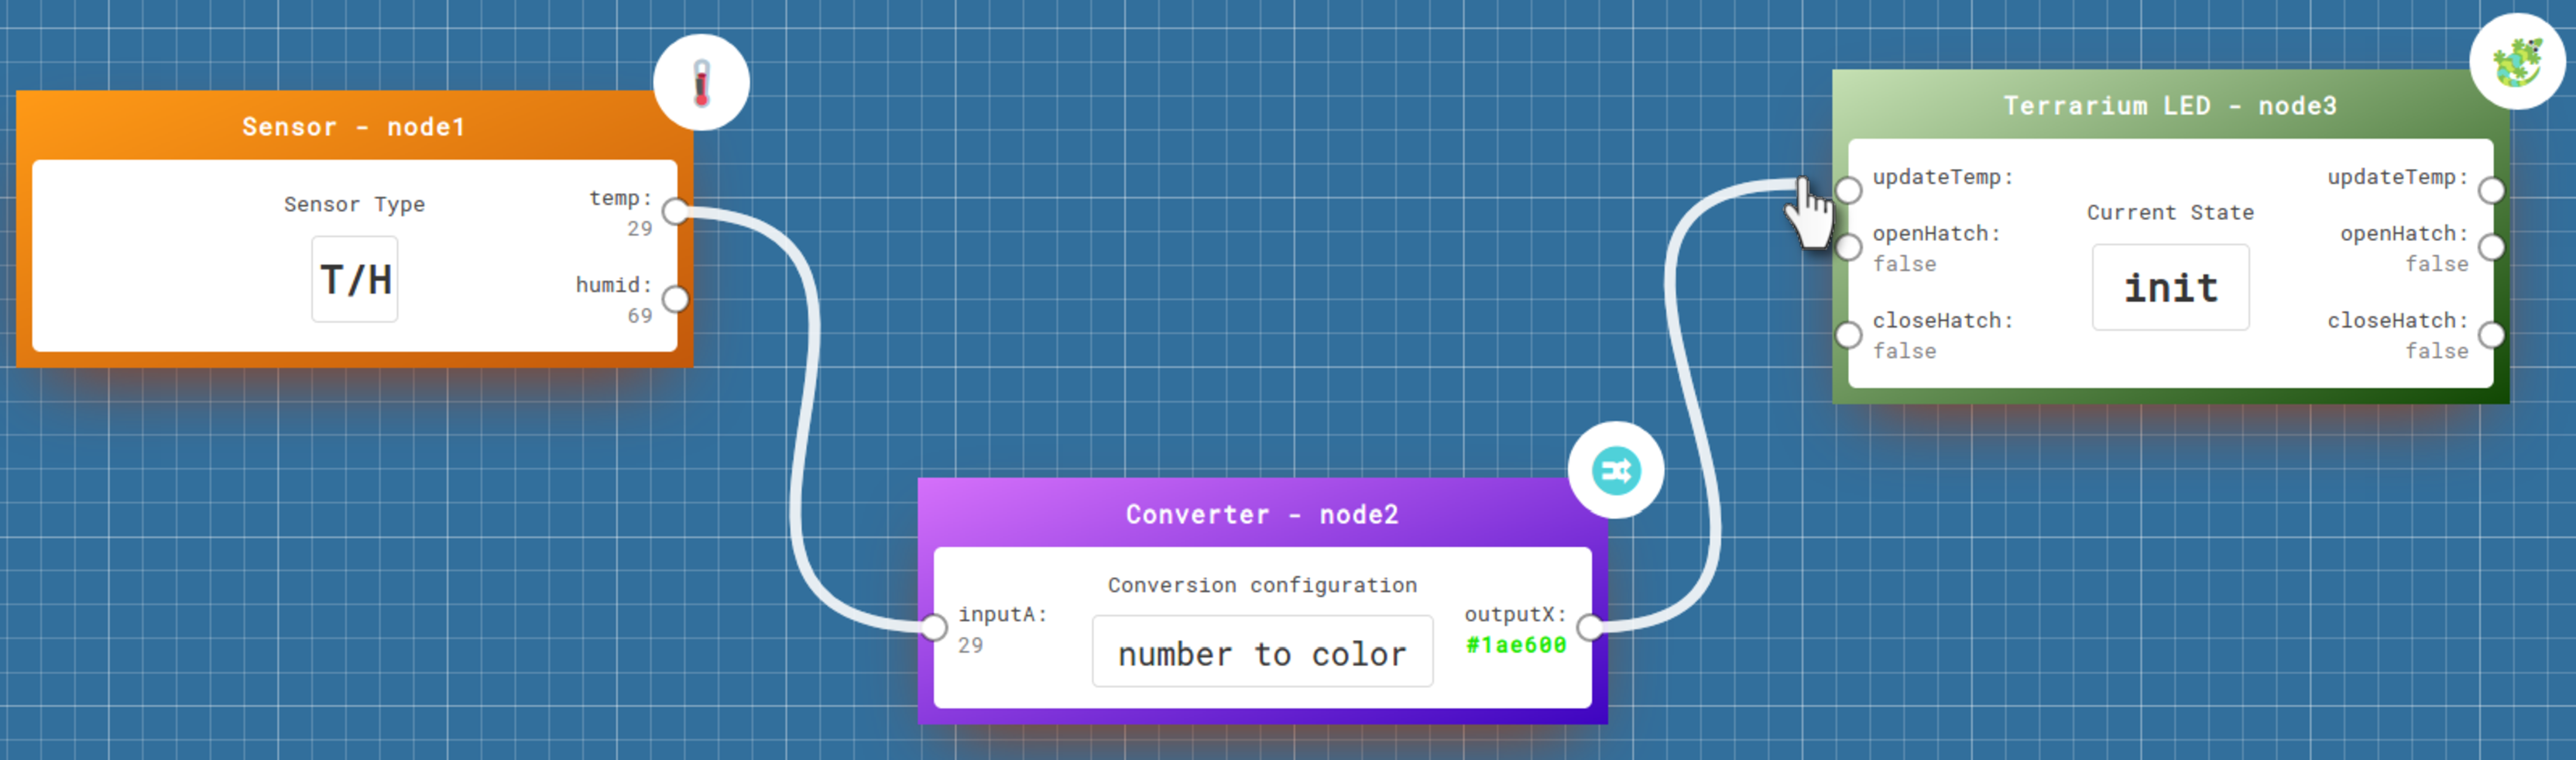
\includegraphics[width=1\textwidth]{bilder/chapter5/screenshotflows.pdf}
  \caption{Screenshot des flowws-Prototyps}
  \label{fig:genericnode}
\end{figure}

Für die Evaluation wurde im Zuge dieser Thesis eine prototypische Implementierung von flowws erstellt. Der Prototyp kann die grundlegenden Elemente (Sensor-, Aktor- und Funktionsknoten, Verbindungen) von flowws darstellen und animieren. Darüber hinaus, lassen sich die Elemente miteinander kombinieren und die Signalverarbeitung des Graphen simulieren.

Der Sourcecode wurde als \textit{Webapp} mit dem React-Framework\footnote{\url{https://reactjs.org/} - besucht September 2018} erstellt und steht in einem \textit{Github-Repository}\footnote{\url{https://github.com/chrbrt/flowws} - besucht September 2018} zur freien Verfügung und Erweiterung.
\section{Durchführung der qualitativen Evaluation}

Die Durchführung des Benutzertests geschah mit drei Personen, von denen zwei Personen, Designer (Master of Arts und Diplom). Die andere Person arbeitet im Bereich der \textit{Business-Communication}/Marketing (\textit{Master of Arts}), besitzt allerdings praktische Erfahrung im Bereich \textit{Product-Design} durch aktiver Beteiligung an mehreren Design-Projekten. Sie sind alle weiblich, zwischen 22-35 Jahren alt, und besitzen umfangreiches Wissen über Designmehthoden (bspw. \textit{Rapid-Prototyping}, \textit{Design-Thinking}, etc.). Die Erfahrung der Benutzergruppe im Bereich \ac{IoT} und \textit{Soft\-ware-Engineering} ist gering und reicht von ''\textit{unbedarft}'' bis ''\textit{Grundkenntnisse} mit Arduino''. Die Benutzergruppe reflektiert somit den Charakter der Persona ''Laura'' (siehe Kapitel \ref{sec:persona}) gut.

\subsection*{Verständnis Datenfluss-Komponente des flowws-Graphen}
Die Datenfluss-Kom\-po\-nen\-te ist das initiale Element, dass der Benutzer bei flowws erblickt. Es wurde die \textit{funktionale Aussagekraft}, \textit{Sichtbarkeit}, die \textit{fortwährende Evaluation} des Programmes und die Qualität der \textit{Abstraktionen} (siehe \ref{tab:cognitivedimensions}) der einzelnen Knoten evaluiert. Folgende Beobachtungen wurden gemacht: 
\begin{itemize}
    \item Zwei von drei Probanden konnten die virtuellen Knoten mit denen der physischen Knoten abgleichen.
    \item Alle Probanden identifizieren, das Signale zwischen den einzelnen Knoten gesendet werden.
    \item Eine der Probanden gab an, sie dachten, dass Funktionsknoten auch physische Knoten repräsentieren (z.B. \textit{Timer}-Knoten).
    \item Alle Probanden konnten durch das Vergleichen von In- und Output, auf die Funktionen der Knoten schließen.
    \item Zwei der drei Probanden konnte die Arbeitsweise des ersten Datenflussgraphen deuten, ohne vom Gutachter darauf hingewiesen zu werden. Der Graphen des zweiten Szenarios konnte nur teilweise gedeutet werden. Erst nach Erläuterung des Zieles des Prototypen, konnten der Sinn, der einzelnen Elemente gedeutet werden. 
    \item Die Person mit der meisten Erfahrung in Software-Engineering wurde durch ihr eigenes Wissen von Kontrollstrukturen abgelenkt. Sie deutete die Verbindungen zwischen den Knoten als bedingte Verzweigungen. Die zwei anderen Probanden besaßen aufgrund ihrer naiveren Betrachtungsweise, weniger Probleme, die Funktion des Graphen zu identifizieren.
    \item Ein Proband bemängelte, dass generische Knoten nicht benannt sind (bspw. anstatt ''Taster'', ''Taster für Terrariumöffnung'').
\end{itemize}

\subsection*{Verständnis für Aktoren/\ac{FSM}} 
Die Steuerung der Aktor-\ac{FSM} ist die zweite Säule des flowws-Konzepts. Ähnlich wie bei der Datenfluss-Komponente, wurden die Komponenten des Aktors auf Basis der gleichen \ac{CD} evaluiert. Die Probanden bemerkten Folgendes:
\begin{itemize}
    \item Alle Probanden konnten den Aktor als solchen identifizieren.
    \item Ohne Einweisung, konnten die Probanden nur wenig mit der Darstellung der \ac{FSM} anfangen. Nach kurzer Erläuterung, wurde das Prinzip von allen Probanden angenommen.
    \item Die Benutzer hatten Probleme mit der rein symbolischen Benennung von Zuständen. -- ''\textit{Warum ist 'Klappe geöffnet' ein Zustand innerhalb des LED Aktors?}'' 
    \item Ein Proband hat erwartet, dass die zeitliche Steuerung innerhalb des Aktors selbst stattfindet, anstatt in einem separaten Funktionsknoten.
    \item Ein Proband konnte den Rückgabewert (\texttt{return(<wert>)}) dem Ausgang des Aktors zuordnen, alle anderen Probanden hatten Probleme mit dem Konzept eines Rückgabewerts.
    \item Nach einer Erläuterung konnten zwei von drei Probanden das Verhalten des Aktors auf willkürliche Eingangssignale vorhersagen. Dabei beschrieben sie implizit die Fähigkeit von \acp{FSM}, Signale zu priorisieren.
\end{itemize}

\subsection*{Verständnis für Darstellung von flowws}
\begin{itemize}
    \item Farbliche Aufteilung der Knoten in Sensor, Funktion und Aktor wurde von allen Benutzern sofort unterbewusst angenommen.
    \item Die Farben der Aktor-Eingänge sollten mit den Farben der Übergängen übereinstimmen.
    \item Animationen beim Ändern von In- und Output-werten sehr hilfreich. Auch die Animation der Verbindungen half den Probanden bei dem Nachverfolgen der Daten.
    \item Animationen sind zum Teil zu schnell. -- ''\textit{Ich habe gesehen, dass sich etwas verändert hat, aber nicht genau was.}''
    \item Eine Funktion zum pausieren der Sensoren wäre hilfreich.
    \item Die Darstellung und Animationen von flowws erinnern laut Probanden an Rohrleitungen und an Dia\-lyse\-ge\-räte.    
    \item Der Verlust eines Indexes, mit sämtlichen Funktionsknoten machte einen einen Probanden unsicher, da keine Knoten zum Vergleichen bereitstanden. Ein Index würde einen besseren Gesamtkontext für die Funktionsknoten bieten. 
\end{itemize}
\subsection*{Sonstige Bemerkungen} 
\begin{itemize}
    \item Zwei von drei Probanden fingen an, mit der Konfigurationen der Funktionsknoten zu explorieren, ohne dass sie dazu aufgefordert wurden und der Prototyp dieses nur im geringen Maße unterstützt.
    \item Die Probanden besitzen Schwierigkeiten mit nicht-deskriptiven Daten. Ein Proband konnte nichts mit einem Helligkeitswerte von 1.0 des LED-Aktors anfangen, da sie die prozentuale Skala der Eigenschaft nicht intuitiv herleiten konnte.
    \item Einem der Probanden war es möglich die Fehlkonfiguration eines Funktionsknotens, durch den Gutachter, auszumachen.
\end{itemize}

\section{Wertung der Ergebnisse}

\subsection{Erfüllung der Anforderungen}
Die Evaluation hat neben dem Beweis der Hypothese, auch Aufschluss über die Erfüllung der Anforderungen aus Kapitel \ref{sec:anforderungen} gegeben. Im Folgenden wird im Anbetracht der Ergebnisse der Nutzertests diskutiert, in wie weit flowws den Anforderungen gerecht wird und welche Anforderungen noch weitere Evaluation benötigen.

\subsubsection{Erfüllen von funktionale Anforderungen}
Die funktionalen Anforderungen aus Kapitel \ref{subsec:fanf} bezogen sich hauptsächlich auf die Verarbeitung von Daten. Vergleichs-, bool'sche und zeitgesteuerte Operationen (siehe \hyperref[tab:fanf]{FA\#1-3}) sowie die Konvertierung von Signalen (\hyperref[tab:fanf]{FA\#7}) werden von Funktionsknoten abgebildet. Das Auslesen und Anzeigen von Sensordaten (\hyperref[tab:fanf]{FA\#4}) geschieht automatisch über die Sensorknoten. Das Konzept zum Ansteuern von Aktoren und das Programmieren von Aktoren (\hyperref[tab:fanf]{ FA\#5} u. \hyperref[tab:fanf]{ FA\#6}) wurden in Kapitel \ref{subsubsec:evebtkonsumierung} und Kapitel \ref{FSMkreieren} ausführlich beschrieben.

\subsubsection{Erfüllen nicht funktionalen Anforderungen}
\paragraph{NFA \#0: Parallel und Sequentielles....} Durch das Konzeptmodell von flowws, welches Datenfluss- und \ac{FSM}-Programmierung kombiniert konnte diese Anforderung erfüllt werden. Die Nutzertests haben angedeutet, dass potentielle Endnutzer paralleles und sequentielles Verhalten, ohne hohen kognitiven Aufwand innerhalb von flowws, begreifen können.

\paragraph{NFA \#1: Daten und State ...} flowws visualisiert Daten und Zustand des Programms an mehreren Stellen. Jeder Knoten zeigt seine aktuellen Ein- und Ausgangs Daten an, der Fluss von Daten wird animiert und der Zustand von Aktoren wird dargestellt (siehe Kapitel\ref{sec:graphischesmodell}). Dadurch entsteht ein Gefühl von dynamik, die es dem Endnutzer erlaubt zu Laufzeit das Verhalten des Programms nachzuvollziehen. Dies wurde von den Nutzertests bestätigt.

\paragraph{NFA \#2: Schneller erlernbar...} Durch die visuelle Darstellung von flowws wird sich erhofft, dass das visuelle Denken von Menschen unterstützt wird und somit sich der Lernaufwand reduziert. Die Nutzertests haben Aufschluss über die Verständlichkeit von flowws geliefert. Um einen besseren Aufschluss über die Erlernbarkeit von flowws zu erreichen, müssen weitere Prototypen gebaut werden, welche es Probanden erlauben eigene Graphen zu modellieren.

\paragraph{NFA \#3: Schnelle modifzierung...} Die Komponenten von flowws (Sensoren, Funktionen, Aktoren) sind allesamt in einzelne Knoten gekapselt und durch klar definierte Schnittstellen miteinander verbunden. Funktions- und Aktorknoten lassen sich noch individuell konfigurieren. Dies lädt den Endnutzer dazu ein, Knoten auszutauschen und zügig mehrere Alternativen zu einem bestehenden flowws-Graphen zu erproben. Dieses Verhalten konnte auch schon in den Nutzertests nachgewiesen werden.

\paragraph{NFA \#4: Fehlerprävention} Der größte Teil der Programmierung in flowws stellt das Verbinden von Knoten. flowws versucht durch kontextuelles Markieren von kompatiblen Schnittstellen und dem kontextuellen Auswählen von kompatiblen Funktionsknoten, die Fehlerzahl im Voraus zu reduzieren. 

\paragraph{NFA \#5: Erweiterbarkeit von Komponenten} flowws kann auf zwei Ebenen von Experten erweitert werden: zum einen durch benutzerdefinierter Logik von Funktionsknoten und zum anderen durch definieren von Aktorfunktionen. Diese beiden Gegebenheiten sollten es fortgeschrittenen Endnutzern erlauben, eine größere Bandbreite von Szenarien abzudecken. Des Weiteren ist flowws \textit{Open Source} und somit von Software-Ingenieuren erweiterbar und anpassbar.


\section{Erfüllung der Anforderungen und Ziele}
- Erfüllung von funktionalen Anforderungen
- Erfüllung von nicht funktionalen Anforderungen
- Erfüllung von Zielen



